% Options for packages loaded elsewhere
\PassOptionsToPackage{unicode}{hyperref}
\PassOptionsToPackage{hyphens}{url}
%
\documentclass[
]{article}
\usepackage{lmodern}
\usepackage{amssymb,amsmath}
\usepackage{ifxetex,ifluatex}
\ifnum 0\ifxetex 1\fi\ifluatex 1\fi=0 % if pdftex
  \usepackage[T1]{fontenc}
  \usepackage[utf8]{inputenc}
  \usepackage{textcomp} % provide euro and other symbols
\else % if luatex or xetex
  \usepackage{unicode-math}
  \defaultfontfeatures{Scale=MatchLowercase}
  \defaultfontfeatures[\rmfamily]{Ligatures=TeX,Scale=1}
\fi
% Use upquote if available, for straight quotes in verbatim environments
\IfFileExists{upquote.sty}{\usepackage{upquote}}{}
\IfFileExists{microtype.sty}{% use microtype if available
  \usepackage[]{microtype}
  \UseMicrotypeSet[protrusion]{basicmath} % disable protrusion for tt fonts
}{}
\makeatletter
\@ifundefined{KOMAClassName}{% if non-KOMA class
  \IfFileExists{parskip.sty}{%
    \usepackage{parskip}
  }{% else
    \setlength{\parindent}{0pt}
    \setlength{\parskip}{6pt plus 2pt minus 1pt}}
}{% if KOMA class
  \KOMAoptions{parskip=half}}
\makeatother
\usepackage{xcolor}
\IfFileExists{xurl.sty}{\usepackage{xurl}}{} % add URL line breaks if available
\IfFileExists{bookmark.sty}{\usepackage{bookmark}}{\usepackage{hyperref}}
\hypersetup{
  hidelinks,
  pdfcreator={LaTeX via pandoc}}
\urlstyle{same} % disable monospaced font for URLs
\usepackage{color}
\usepackage{fancyvrb}
\newcommand{\VerbBar}{|}
\newcommand{\VERB}{\Verb[commandchars=\\\{\}]}
\DefineVerbatimEnvironment{Highlighting}{Verbatim}{commandchars=\\\{\}}
% Add ',fontsize=\small' for more characters per line
\newenvironment{Shaded}{}{}
\newcommand{\AlertTok}[1]{\textcolor[rgb]{1.00,0.00,0.00}{\textbf{#1}}}
\newcommand{\AnnotationTok}[1]{\textcolor[rgb]{0.38,0.63,0.69}{\textbf{\textit{#1}}}}
\newcommand{\AttributeTok}[1]{\textcolor[rgb]{0.49,0.56,0.16}{#1}}
\newcommand{\BaseNTok}[1]{\textcolor[rgb]{0.25,0.63,0.44}{#1}}
\newcommand{\BuiltInTok}[1]{#1}
\newcommand{\CharTok}[1]{\textcolor[rgb]{0.25,0.44,0.63}{#1}}
\newcommand{\CommentTok}[1]{\textcolor[rgb]{0.38,0.63,0.69}{\textit{#1}}}
\newcommand{\CommentVarTok}[1]{\textcolor[rgb]{0.38,0.63,0.69}{\textbf{\textit{#1}}}}
\newcommand{\ConstantTok}[1]{\textcolor[rgb]{0.53,0.00,0.00}{#1}}
\newcommand{\ControlFlowTok}[1]{\textcolor[rgb]{0.00,0.44,0.13}{\textbf{#1}}}
\newcommand{\DataTypeTok}[1]{\textcolor[rgb]{0.56,0.13,0.00}{#1}}
\newcommand{\DecValTok}[1]{\textcolor[rgb]{0.25,0.63,0.44}{#1}}
\newcommand{\DocumentationTok}[1]{\textcolor[rgb]{0.73,0.13,0.13}{\textit{#1}}}
\newcommand{\ErrorTok}[1]{\textcolor[rgb]{1.00,0.00,0.00}{\textbf{#1}}}
\newcommand{\ExtensionTok}[1]{#1}
\newcommand{\FloatTok}[1]{\textcolor[rgb]{0.25,0.63,0.44}{#1}}
\newcommand{\FunctionTok}[1]{\textcolor[rgb]{0.02,0.16,0.49}{#1}}
\newcommand{\ImportTok}[1]{#1}
\newcommand{\InformationTok}[1]{\textcolor[rgb]{0.38,0.63,0.69}{\textbf{\textit{#1}}}}
\newcommand{\KeywordTok}[1]{\textcolor[rgb]{0.00,0.44,0.13}{\textbf{#1}}}
\newcommand{\NormalTok}[1]{#1}
\newcommand{\OperatorTok}[1]{\textcolor[rgb]{0.40,0.40,0.40}{#1}}
\newcommand{\OtherTok}[1]{\textcolor[rgb]{0.00,0.44,0.13}{#1}}
\newcommand{\PreprocessorTok}[1]{\textcolor[rgb]{0.74,0.48,0.00}{#1}}
\newcommand{\RegionMarkerTok}[1]{#1}
\newcommand{\SpecialCharTok}[1]{\textcolor[rgb]{0.25,0.44,0.63}{#1}}
\newcommand{\SpecialStringTok}[1]{\textcolor[rgb]{0.73,0.40,0.53}{#1}}
\newcommand{\StringTok}[1]{\textcolor[rgb]{0.25,0.44,0.63}{#1}}
\newcommand{\VariableTok}[1]{\textcolor[rgb]{0.10,0.09,0.49}{#1}}
\newcommand{\VerbatimStringTok}[1]{\textcolor[rgb]{0.25,0.44,0.63}{#1}}
\newcommand{\WarningTok}[1]{\textcolor[rgb]{0.38,0.63,0.69}{\textbf{\textit{#1}}}}
\usepackage{graphicx,grffile}
\makeatletter
\def\maxwidth{\ifdim\Gin@nat@width>\linewidth\linewidth\else\Gin@nat@width\fi}
\def\maxheight{\ifdim\Gin@nat@height>\textheight\textheight\else\Gin@nat@height\fi}
\makeatother
% Scale images if necessary, so that they will not overflow the page
% margins by default, and it is still possible to overwrite the defaults
% using explicit options in \includegraphics[width, height, ...]{}
\setkeys{Gin}{width=\maxwidth,height=\maxheight,keepaspectratio}
% Set default figure placement to htbp
\makeatletter
\def\fps@figure{htbp}
\makeatother
\usepackage[normalem]{ulem}
% Avoid problems with \sout in headers with hyperref
\pdfstringdefDisableCommands{\renewcommand{\sout}{}}
\setlength{\emergencystretch}{3em} % prevent overfull lines
\providecommand{\tightlist}{%
  \setlength{\itemsep}{0pt}\setlength{\parskip}{0pt}}
\setcounter{secnumdepth}{-\maxdimen} % remove section numbering

\date{}

\begin{document}

\hypertarget{header-n0}{%
\section{SE-344}\label{header-n0}}

\hypertarget{header-n2}{%
\subsection{Assignment Final Report}\label{header-n2}}

\hypertarget{header-n3}{%
\subsubsection{概述}\label{header-n3}}

\hypertarget{header-n4}{%
\paragraph{第一部分:技术框架}\label{header-n4}}

\hypertarget{header-n5}{%
\subparagraph{GLFW}\label{header-n5}}

由于 GLFW 相较于 FreeGLUT 提供了更接近底层的 Shader
支持,因此第一部分涉及到法线贴图的动画将基于 GLFW 开发。

使用的 GLFW 版本是 \texttt{3.3}。

\hypertarget{header-n8}{%
\subparagraph{FreeGLUT}\label{header-n8}}

由于这一 Utility Toolkit 提供了封装过的大量的实用工具函数,极大地简化了
OpenGL 的开发进程,因此後续一些相对简单的动画制作将基于 FreeGLUT 完成。

使用的 FreeGLUT 版本是 \texttt{3.2.1}。

\hypertarget{header-n11}{%
\subparagraph{SOIL}\label{header-n11}}

由于本次作业涉及到大量背景和材质图片的读取,而 OpenGL 本身没有提供除
\texttt{.bmp} 格式之外的图片读取器。因此,引入了 SOIL 库作为
\texttt{.png} 格式素材的读取器。

\hypertarget{header-n13}{%
\subparagraph{编译环境}\label{header-n13}}

使用的操作系统是 Windows 10 x64 LTSC 1809 (\texttt{17763.737})。

使用的 IDE 是 Visual Studio 2019 Community (\texttt{16.2.4})。

\hypertarget{header-n16}{%
\subparagraph{编程语言}\label{header-n16}}

为了方便管理及控制复杂度,本次大作业的主体部分被拆分成了四个基于 OpenGL
的程序,每一个对应故事情节中的一部分。他们分别基于 GLFW 和
FreeGLUT,均以 C++ 写成。

为了方便展示观看,还使用 C\#
写了一个调度器。她将按照故事剧情依次进行调度,同时播放适当的音频以渲染气氛。

\hypertarget{header-n19}{%
\paragraph{第二部分:运行时截图}\label{header-n19}}

\hypertarget{header-n20}{%
\subparagraph{Intro 页面}\label{header-n20}}

\begin{figure}
\centering
\includegraphics{/Users/yue/Documents/GitHub/2019-2020-autumn-semester/SE-344/submissions/ass4-ng-x/report/report.assets/1.intro.png}
\caption{}
\end{figure}

\begin{quote}
静态片头画面。
\end{quote}

\hypertarget{header-n24}{%
\subparagraph{Notebook 页面}\label{header-n24}}

\begin{figure}
\centering
\includegraphics{/Users/yue/Documents/GitHub/2019-2020-autumn-semester/SE-344/submissions/ass4-ng-x/report/report.assets/2.book.png}
\caption{}
\end{figure}

\begin{quote}
笔记本翻转着进入镜头。同时,可以感受到光线带来的表面凹凸效果。
\end{quote}

\begin{figure}
\centering
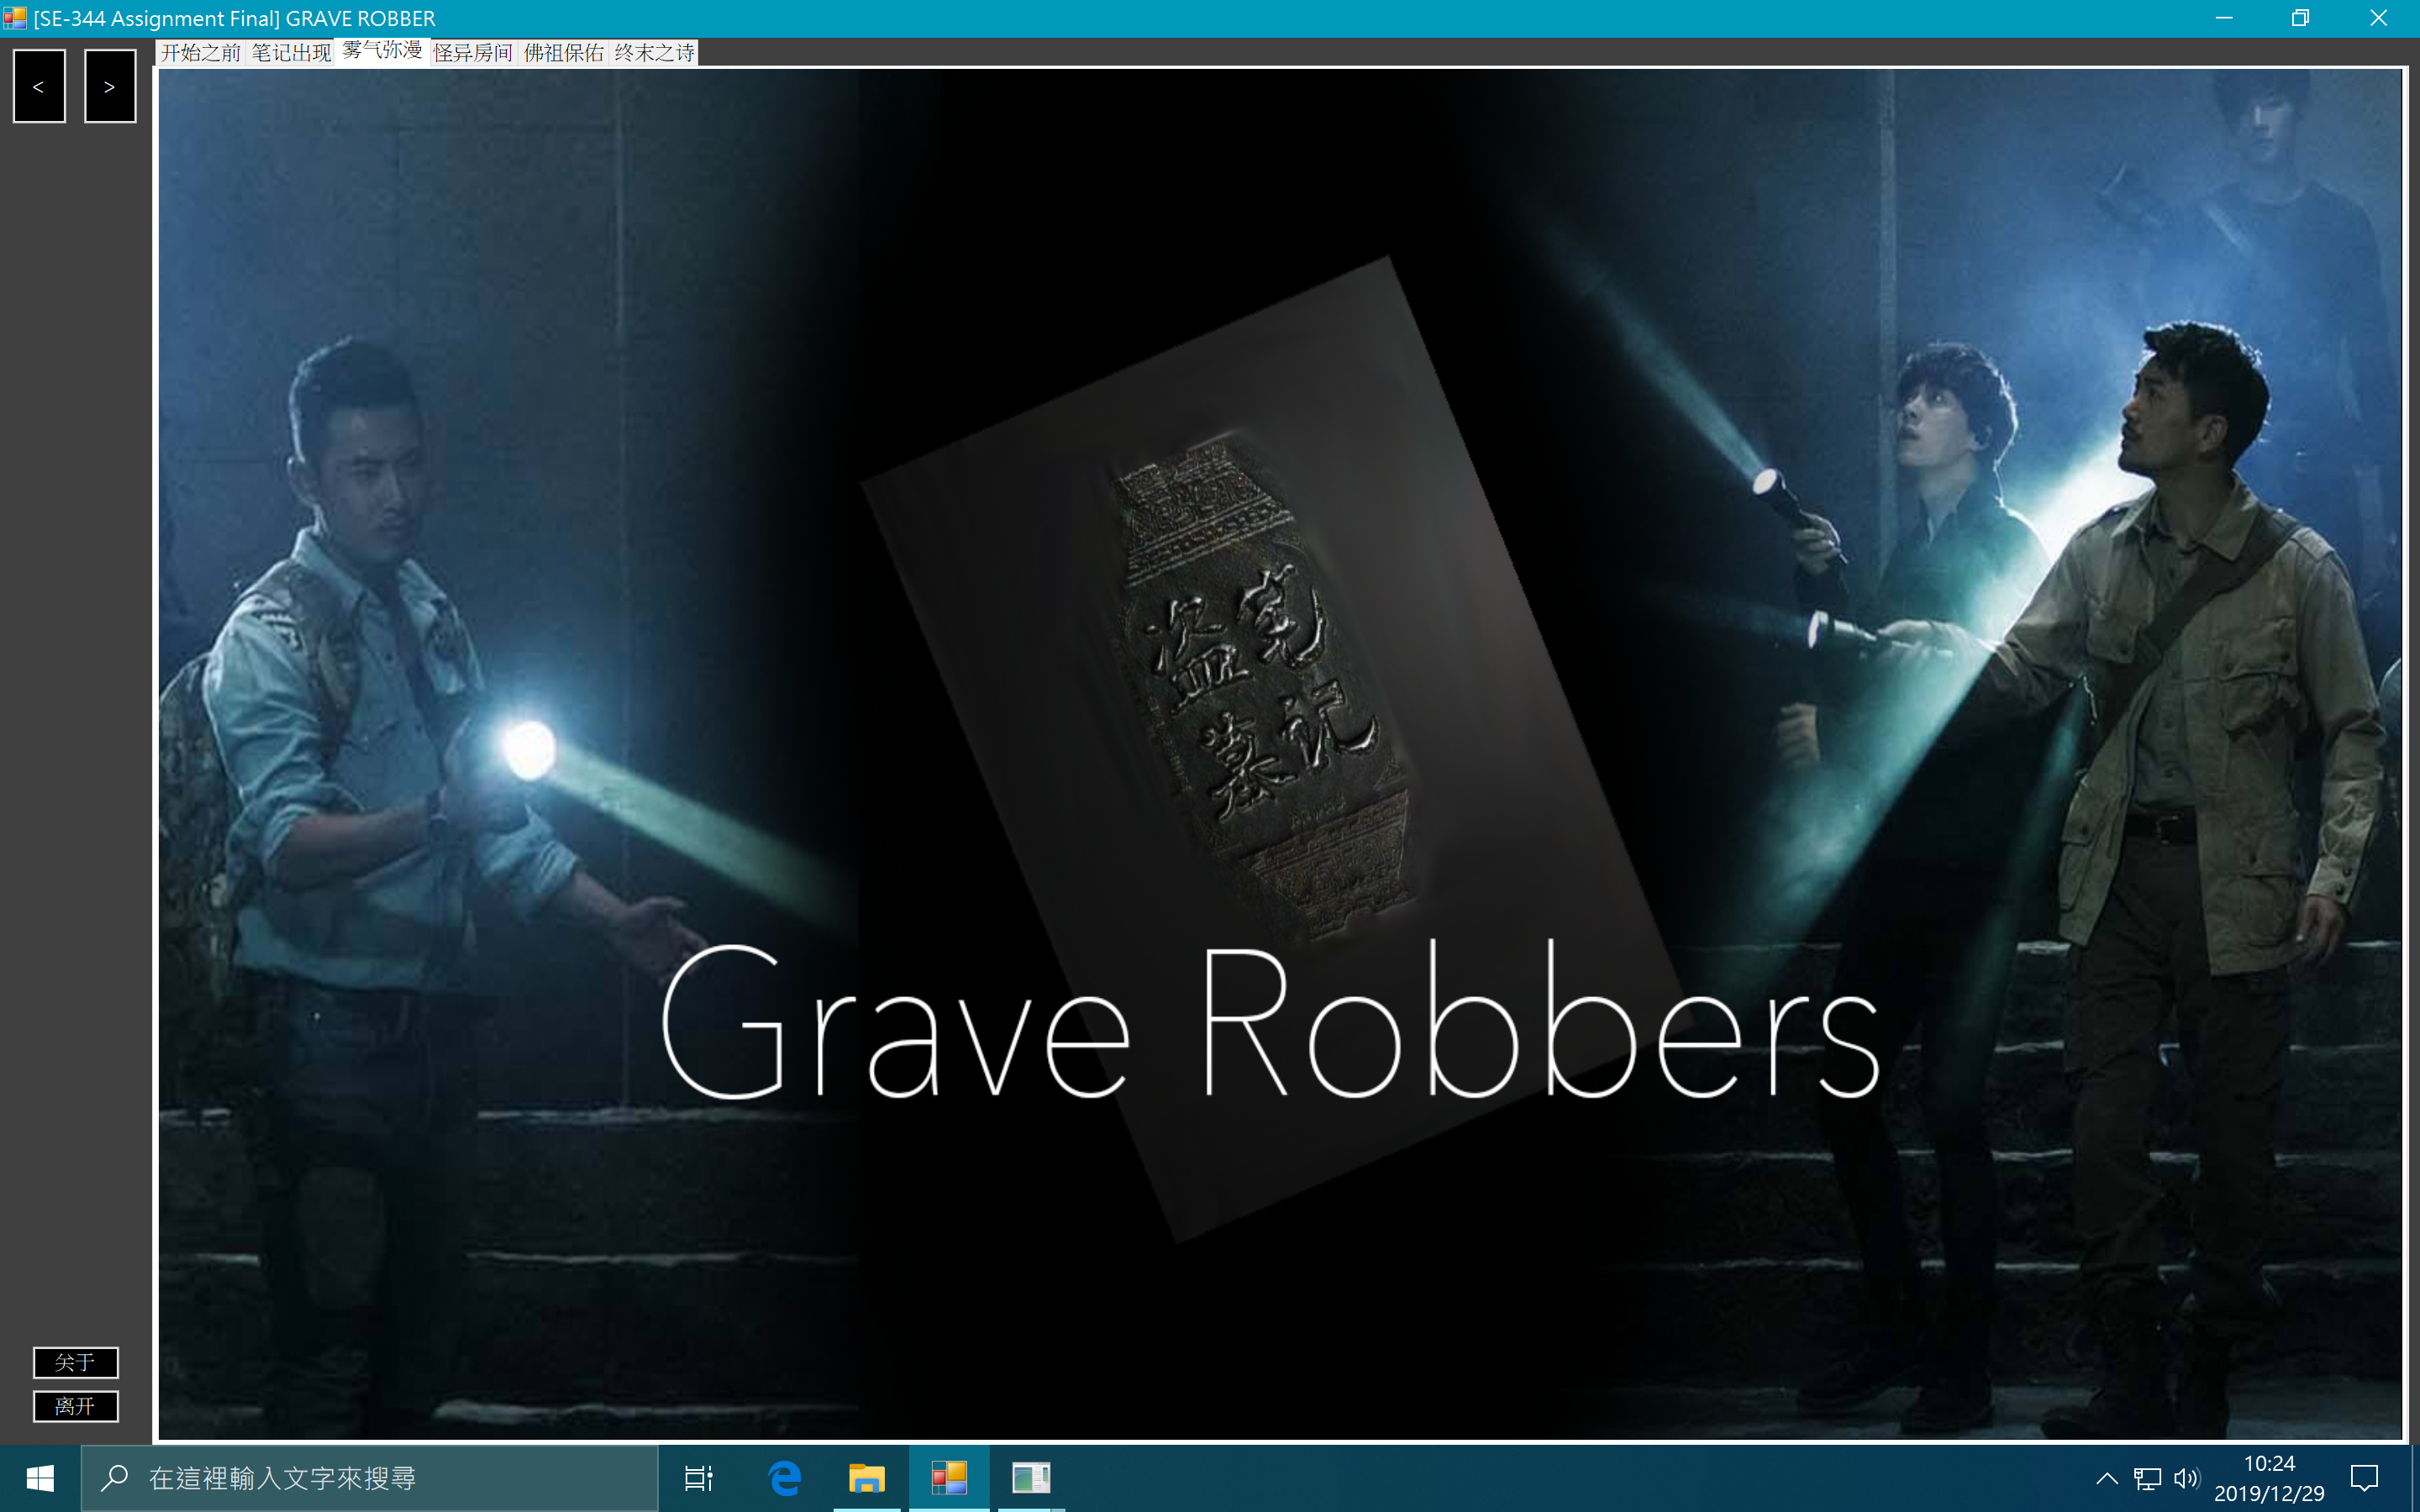
\includegraphics{/Users/yue/Documents/GitHub/2019-2020-autumn-semester/SE-344/submissions/ass4-ng-x/report/report.assets/3.room.png}
\caption{}
\end{figure}

\begin{quote}
笔记本渐渐飘远,进入下一场景。
\end{quote}

\hypertarget{header-n31}{%
\subparagraph{Smoke 页面}\label{header-n31}}

\begin{figure}
\centering
\includegraphics{/Users/yue/Documents/GitHub/2019-2020-autumn-semester/SE-344/submissions/ass4-ng-x/report/report.assets/4.fog.and.book.png}
\caption{}
\end{figure}

\begin{quote}
具有粒子效果的迷雾扩散并遮盖了笔记本。
\end{quote}

\begin{figure}
\centering
\includegraphics{/Users/yue/Documents/GitHub/2019-2020-autumn-semester/SE-344/submissions/ass4-ng-x/report/report.assets/5.fog.png}
\caption{}
\end{figure}

\begin{quote}
笔记本已经看不见了。
\end{quote}

\begin{figure}
\centering
\includegraphics{/Users/yue/Documents/GitHub/2019-2020-autumn-semester/SE-344/submissions/ass4-ng-x/report/report.assets/6.fog.vanished.png}
\caption{}
\end{figure}

\begin{quote}
迷雾散去,出现了一间暗室。
\end{quote}

\hypertarget{header-n41}{%
\subparagraph{Darkroom 页面}\label{header-n41}}

\begin{figure}
\centering
\includegraphics{/Users/yue/Documents/GitHub/2019-2020-autumn-semester/SE-344/submissions/ass4-ng-x/report/report.assets/7.mysterious.room.png}
\caption{}
\end{figure}

\begin{quote}
过场静态图片。进入下一场景。
\end{quote}

\begin{figure}
\centering
\includegraphics{/Users/yue/Documents/GitHub/2019-2020-autumn-semester/SE-344/submissions/ass4-ng-x/report/report.assets/8.dark.room.png}
\caption{}
\end{figure}

\begin{quote}
暗室里几乎什么都看不见,除了面前的一堆石头和四面隐隐发光的墙。
\end{quote}

\begin{figure}
\centering
\includegraphics{/Users/yue/Documents/GitHub/2019-2020-autumn-semester/SE-344/submissions/ass4-ng-x/report/report.assets/9.flashlight.png}
\caption{}
\end{figure}

\begin{quote}
按 Space 键打开手电筒,可以看到明显的高光效果和石头表面凹凸不平的效果。

按 W、A、S、D 键调整光源的位置。按 R 键复位。
\end{quote}

\begin{figure}
\centering
\includegraphics{/Users/yue/Documents/GitHub/2019-2020-autumn-semester/SE-344/submissions/ass4-ng-x/report/report.assets/10.exploded.png}
\caption{}
\end{figure}

\begin{quote}
按下 B 键,炸弹从天而降,碰撞到石头之後产生爆炸。
\end{quote}

\hypertarget{header-n55}{%
\subparagraph{Buddha 页面}\label{header-n55}}

\begin{figure}
\centering
\includegraphics{/Users/yue/Documents/GitHub/2019-2020-autumn-semester/SE-344/submissions/ass4-ng-x/report/report.assets/11.buddha.png}
\caption{}
\end{figure}

\begin{quote}
静态过场图片。进入下一场景。
\end{quote}

\begin{figure}
\centering
\includegraphics{/Users/yue/Documents/GitHub/2019-2020-autumn-semester/SE-344/submissions/ass4-ng-x/report/report.assets/12.buddha.low.png}
\caption{}
\end{figure}

\begin{quote}
此时场景仍然在之前的房间里,但相较上一个画面亮度提高了些,视角也有所改变。

初始情况下,模型分辨率很低。

为了更明显地表现出方向感和纵深感,场景中放置了三盏 R、G、B
色的灯光,彼此相隔 \(\frac 1 3\) 个圆摆放。
\end{quote}

\begin{figure}
\centering
\includegraphics{/Users/yue/Documents/GitHub/2019-2020-autumn-semester/SE-344/submissions/ass4-ng-x/report/report.assets/13.buddha.medium.png}
\caption{}
\end{figure}

\begin{quote}
模型在运行时动态地加载并使用了中等分辨率的模型。

可以看出此时模型表面光滑了一些。
\end{quote}

\begin{figure}
\centering
\includegraphics{/Users/yue/Documents/GitHub/2019-2020-autumn-semester/SE-344/submissions/ass4-ng-x/report/report.assets/14.buddha.high.png}
\caption{}
\end{figure}

\begin{quote}
模型在运行时动态地加载并使用了高分辨率的模型。

此时模型的表面光滑了不少,表面带着银色的光泽。
\end{quote}

\begin{figure}
\centering
\includegraphics{/Users/yue/Documents/GitHub/2019-2020-autumn-semester/SE-344/submissions/ass4-ng-x/report/report.assets/15.buddha.finest.png}
\caption{}
\end{figure}

\begin{quote}
模型在运行时动态地加载并使用了最高分辨率的模型。

此时模型的表面已经相当光滑了,表面还带着金色的光泽。
\end{quote}

\hypertarget{header-n76}{%
\subparagraph{Outro 页面}\label{header-n76}}

\begin{figure}
\centering
\includegraphics{/Users/yue/Documents/GitHub/2019-2020-autumn-semester/SE-344/submissions/ass4-ng-x/report/report.assets/16.fin.png}
\caption{}
\end{figure}

\begin{quote}
展示了开发过程中引用的第三方库以及参考网站。

非常感谢。
\end{quote}

\hypertarget{header-n81}{%
\paragraph{第三部分:操作说明}\label{header-n81}}

\begin{itemize}
\item
  在 Supervisor 外壳程序中,可点按左下角的「关于」按钮来查看信息。
\item
  在 Supervisor 外壳程序中,可点按左下角的「离开」按钮来结束程序。
\item
  在 Supervisor 外壳程序中,可以通过点按左上角的 \texttt{\textless{}} 和
  \texttt{\textgreater{}} 按钮在不同页面之间切换。
\item
  在 Supervisor 外壳程序中,还可以通过点按屏幕顶部的 Tab
  菜单页来切换分页。
\item
  在 Darkroom 页面子程序中,点按空格键即可打开「手电筒」。
\item
  在 Darkroom 页面子程序中,在手电筒开启的状态下可通过按 W、A、S、D
  来调整灯光位置。
\item
  在 Darkroom 页面子程序中,在手电筒开启的状态下可通过按 R
  来将灯光复位。
\item
  在 Darkroom 页面子程序中,在手电筒开启的状态下可通过按 B 来引爆炸弹。
\end{itemize}

\hypertarget{header-n99}{%
\subsubsection{详细}\label{header-n99}}

\hypertarget{header-n100}{%
\paragraph{第一部分:笔记出现}\label{header-n100}}

\hypertarget{header-n101}{%
\subparagraph{模型建构}\label{header-n101}}

这一步骤中需要的模型相对简单:只是一个长宽比为
\(\sqrt 2 : 1\)、厚度随意的六面立方体而已。为了简单起见,不采用从
\texttt{.obj} 或 \texttt{.ply}
文件中读取模型的做法,而是直接将模型顶点数据硬编码到源代码中。

\begin{quote}
此部分对应的源文件为 \texttt{./1-title/source/ModelKits.hpp}。
\end{quote}

模型采用如下的结构体保存:

\begin{Shaded}
\begin{Highlighting}[]
\KeywordTok{typedef} \KeywordTok{struct}\NormalTok{ modelRecord \{}
    \DataTypeTok{float}\NormalTok{* buffer;}
    \DataTypeTok{size_t}\NormalTok{ size;}
\NormalTok{\} * modelRecordT;}
\end{Highlighting}
\end{Shaded}

\texttt{float} 数组中,八个浮点数编为一组表示一个顶点;分别是 3
个顶点坐标、3 个顶点法向量和 2 个顶点纹理坐标 u、v。

正方体有六个面;每个面需要两个三角形拼凑而成。每个三角形有三个顶点(废话)。因此数组中的浮点数个数为
\(6 \times 2 \times 3 \times 8 = 288\)。

由于 \texttt{float*} 类型无法携带数组大小信息,因此将 \texttt{size}
包装在结构体中一并传递给渲染器。

\hypertarget{header-n110}{%
\subparagraph{材质制作}\label{header-n110}}

Assignment Final 中提供的贴图并非是标准的 Normal Mapping
所需的材质。标准材质中的每个像素点的 R、G、B 分量分别对应了法线方向的
x、y、z,其中 z 为垂直纸面向上的方向。

由于大部分材质的起伏都不大,基本都沿着正规的 z
方向,因此反映到材质图片中的 B(蓝色)分量就相对较高,整体色调就偏蓝。

将给出的深度图转换为法线贴图的方式很多;这里采用了 \texttt{CrazyBump}
软件来实现这一转换。

转换前后的图片如图所示。

\begin{figure}
\centering
\includegraphics{/Volumes/Macintosh HD (Sierra)/Users/yue/Documents/GitHub/2019-2020-autumn-semester/SE-344/submissions/ass4-ng-x/report/report.assets/origin_and_nrm.png}
\caption{}
\end{figure}

\hypertarget{header-n116}{%
\subparagraph{材质加载}\label{header-n116}}

为了在保证图片质量的前提下尽量减小文件体积,所有贴图一律采用
\texttt{.png} 格式保存。

首先,使用 \texttt{glGenTextures} 函数初始化一类材质 ID。用
\texttt{glActiveTexture} 函数将其在上下文中激活。

接着,通过 \texttt{stbi\_load} 函数即可将贴图文件读取到
\texttt{unsigned\ char*\ buffer} 缓冲区中。

随后,使用 \texttt{glTexImage2D} 函数即可使用缓冲区初始化材质。

最后,别忘了用 \texttt{stbi\_image\_free} 释放缓冲区,以免内存泄漏。

通过这种操作,依次引入三种材质:一种是 \texttt{title.png}
对应的一般表面贴图;一种是 \texttt{title\_spec.png}
对应的反射光贴图;一种是 \texttt{title\_NRM.png} 对应的法线贴图。

\begin{quote}
反射光贴图通过明/暗的区域来指定物体表面反射光的强度,以增强真实感。
\end{quote}

\hypertarget{header-n125}{%
\subparagraph{绘制模型}\label{header-n125}}

GLFW 的模型绘制没有 FreeGLUT 那样良好的封装。因此步骤相对来说复杂一些。

由于这里需要大量空间向量的计算,因此引入了 \texttt{glm} 库来辅助。

为了实现镜头逐渐拉远的效果,使用下面的代码来计算视角向量:

\begin{Shaded}
\begin{Highlighting}[]
\ControlFlowTok{if}\NormalTok{ ( zoomOutSpeed > }\FloatTok{0.01}\BuiltInTok{f}\NormalTok{ ) \{}
\NormalTok{  zoomOutSpeed *= }\FloatTok{0.5}\BuiltInTok{f}\NormalTok{;}
\NormalTok{\}}

\NormalTok{view = glm::translate( view, glm::vec3( }\FloatTok{0.0}\BuiltInTok{f}\NormalTok{, }\FloatTok{0.0}\BuiltInTok{f}\NormalTok{, -zoomOutSpeed ) );}
\end{Highlighting}
\end{Shaded}

将视角位置向量 \texttt{view} 保存好,稍后会用到。

同时模型还需要自转,因此使用下面的代码来旋转模型:

\begin{Shaded}
\begin{Highlighting}[]
\NormalTok{model = glm::rotate( model, radius, glm::vec3( }\FloatTok{0.5}\BuiltInTok{f}\NormalTok{, }\FloatTok{0.1}\BuiltInTok{f}\NormalTok{, }\FloatTok{0.0}\BuiltInTok{f}\NormalTok{ ) );}
\end{Highlighting}
\end{Shaded}

代码将模型向量 \texttt{model} 以 \((0.5, 0.1, 0.0)\) 向量为轴旋转
\texttt{radius} 度。

最后,我们使用 \texttt{glBindVertexArray} 绑定顶点缓冲,并使用
\texttt{glDrawArrays} 绘制模型。

\hypertarget{header-n135}{%
\subparagraph{着色器}\label{header-n135}}

尝试了很多种着色器的实现方法,最终采用的着色器是内嵌在
\texttt{./1-title/rendering/shader.cpp} 中的那一种。

其中顶点着色器相对简单,接受的参数包括一个 \texttt{position}、一个
\texttt{normal} 和一个
\texttt{textureCoordinate}。就是我们上面的顶点缓冲区里的八项内容。

另外还有全局变量 \texttt{projection}、\texttt{view}、\texttt{model} 和
\texttt{normalMatrix},分别代表投影灭点位置、视角位置、模型变换矩阵和法线变换矩阵。

算法只有四行:

\begin{Shaded}
\begin{Highlighting}[]
\NormalTok{gl_Position = projection * view * model * vec4(position, }\FloatTok{2.0}\BuiltInTok{f}\NormalTok{);}
\NormalTok{fragPosition = vec3(model * vec4(position, }\FloatTok{2.0}\BuiltInTok{f}\NormalTok{));}
\NormalTok{outNormal = normalMatrix * normal;}
\NormalTok{textureCoordinates = inTextureCoordinates;}
\end{Highlighting}
\end{Shaded}

最终的位置 \texttt{gl\_Position}
将会由投影点、视角位置、模型位置共同决定。将他们做叉乘来实现计算。

而每个片段的 \texttt{fragPosition} 则直接用 \texttt{model} 和
\texttt{position} 叉乘得到。

真实的法线方向也由输入的法线方向和坐标变换矩阵叉乘得到。

而 \texttt{textureCoordinates} 保持不变,直接传递给片段着色器。

片段着色器就比较复杂了。为了实现凹凸效果,我们需要对法向量开刀,将其改写为
Normal Mapping 的数据。

留意到法线贴图中,R、G、B 分量的取值范围都是
\([0, 1]\);然而实际的法线方向取值范围则是 \([-1, 1]\)。

因此我们必须进行一次线性变换来将其进行重定向,将每一个分量进行
\(\times 2 - 1\) 的操作:

\begin{Shaded}
\begin{Highlighting}[]
\NormalTok{vec3 normalMap = texture(material.emission, textureCoordinates).rgb * }\FloatTok{2.0}\NormalTok{ - }\FloatTok{1.0}\NormalTok{;}
\NormalTok{vec3 normalNormal = normalize(normalMap.rgb);}
\end{Highlighting}
\end{Shaded}

随后,为了计算环境光的颜色,利用下面的公式:

\begin{Shaded}
\begin{Highlighting}[]
\NormalTok{vec3 ambientLight = ambientStrength * lightColor * vec3(texture(material.diffuse, textureCoordinates));}
\end{Highlighting}
\end{Shaded}

计算「光强 × 光色 ×(漫反射系数 结合
贴图坐标)」,即可得到环境光对物体产生的颜色影响。

用同样的方法计算漫反射光的颜色:

\begin{Shaded}
\begin{Highlighting}[]
\NormalTok{vec3 diffuseColor = diffuseStrength * lightColor * vec3(texture(material.diffuse, textureCoordinates));}
\end{Highlighting}
\end{Shaded}

接着,计算反射光的颜色,利用下面的公式:

\begin{Shaded}
\begin{Highlighting}[]
\NormalTok{vec3 specular = specularStrength * lightColor * vec3(texture(material.specular, textureCoordinates));}
\end{Highlighting}
\end{Shaded}

计算「光强 × 光色 ×(镜面反射系数 结合
贴图坐标)」,即可得到反射光对物体产生的颜色影响。

最后,将三种颜色混合在一起,即可得到最终的片段颜色了。

\begin{Shaded}
\begin{Highlighting}[]
\NormalTok{gl_FragColor = vec4(ambientLight + diffuseColor + specular, }\FloatTok{1.0}\BuiltInTok{f}\NormalTok{);}
\end{Highlighting}
\end{Shaded}

\hypertarget{header-n159}{%
\subparagraph{电闪雷鸣}\label{header-n159}}

为了模拟闪电的效果,采用下面这个\sout{随便写的}随机算法来实现:

\begin{Shaded}
\begin{Highlighting}[]
\ControlFlowTok{if}\NormalTok{ ( }\DataTypeTok{int}\NormalTok{( rand_color * }\DecValTok{27544}\NormalTok{ ) % }\DecValTok{13}\NormalTok{ == }\DecValTok{0}\NormalTok{ ) \{}
  \CommentTok{// simulates the storm effect}
\NormalTok{  glClearColor( rand_color, rand_color, rand_color, }\FloatTok{1.0}\BuiltInTok{f}\NormalTok{ );}
\NormalTok{\}}
\ControlFlowTok{else}\NormalTok{ \{}
\NormalTok{  glClearColor( }\FloatTok{0.0}\BuiltInTok{f}\NormalTok{, }\FloatTok{0.0}\BuiltInTok{f}\NormalTok{, }\FloatTok{0.0}\BuiltInTok{f}\NormalTok{, }\FloatTok{1.0}\BuiltInTok{f}\NormalTok{ );}
\NormalTok{\}}
\end{Highlighting}
\end{Shaded}

本质上就是随机用带颜色的笔刷绘制背景而已。配合上外壳程序的声音效果还\sout{勉强}能看。

\hypertarget{header-n163}{%
\paragraph{第二部分:雾气弥漫}\label{header-n163}}

\hypertarget{header-n164}{%
\subparagraph{粒子系统}\label{header-n164}}

这一部分的难点主要是如何模拟真实的雾气弥漫和消散的效果。因此,自行实现了一个简单的、带有增值、耗散的粒子系统。

\begin{quote}
此部分代码参见文件
\texttt{./2-smoke/particles/particle\_generator.hpp}。
\end{quote}

每个粒子具有下面一些属性:

\begin{Shaded}
\begin{Highlighting}[]
\KeywordTok{struct}\NormalTok{ Particle \{}
    \DataTypeTok{float}\NormalTok{ posx, posy;}
    \DataTypeTok{float}\NormalTok{ spdx, spdy;}
    \DataTypeTok{float}\NormalTok{ alpha;}
    \DataTypeTok{bool}\NormalTok{  valid;}
\NormalTok{\};}
\end{Highlighting}
\end{Shaded}

依次为二维空间中的位置、速度,粒子的透明度,以及是否有效的标识位。

由于对于「雾气」来说,粒子存活的时间越久,透明度越低,且半径越大(由于扩散的稀释效应)。

因此将三个变量综合到同一个 \texttt{alpha} 变量中,方便。

关键的粒子系统更新函数主要做下面这些事情:

\begin{itemize}
\item
  按照每个粒子的速度更新其位置;
\item
  令每个粒子在一定范围内随机地失去生命值(对应上面的 \texttt{alpha});
\item
  假如粒子越界、或是生命值降低为 0,则将其从粒子系统中清除;
\item
  随机更新粒子的速度。
\end{itemize}

由于每次更新包含对数组本身的更新,因此采用互斥锁 \texttt{mutex} 来防止
Race。

\hypertarget{header-n184}{%
\subparagraph{绘制粒子}\label{header-n184}}

第二部分的需求很简单,因此也就没有使用 GLFW 的理由了。

核心代码如下:

\begin{Shaded}
\begin{Highlighting}[]
\ControlFlowTok{for}\NormalTok{ ( }\AttributeTok{const} \KeywordTok{auto}\NormalTok{& i : master->particles ) \{}
        \DataTypeTok{float}\NormalTok{ radius      = ( }\FloatTok{1.5}\BuiltInTok{f}\NormalTok{ - i.alpha ) * }\FloatTok{50.0}\BuiltInTok{f}\NormalTok{;}
        \KeywordTok{auto}\NormalTok{  actualAlpha = i.alpha / }\FloatTok{3.0}\BuiltInTok{f}\NormalTok{;}

        \DataTypeTok{double}\NormalTok{ n = }\DataTypeTok{double}\NormalTok{( random_int() % }\DecValTok{6}\NormalTok{ ) + }\DecValTok{6}\NormalTok{;  }\CommentTok{// fragment count}

\NormalTok{        glColor4f( }\FloatTok{1.0}\BuiltInTok{f}\NormalTok{, }\FloatTok{1.0}\BuiltInTok{f}\NormalTok{, }\FloatTok{1.0}\BuiltInTok{f}\NormalTok{, actualAlpha );}
\NormalTok{        glBegin( GL_TRIANGLE_FAN );}
\NormalTok{        _glVertex3f( i.posx, i.posy, }\FloatTok{0.1}\BuiltInTok{f}\NormalTok{ );}

\NormalTok{        glColor4f( }\FloatTok{1.0}\BuiltInTok{f}\NormalTok{, }\FloatTok{1.0}\BuiltInTok{f}\NormalTok{, }\FloatTok{1.0}\BuiltInTok{f}\NormalTok{, }\FloatTok{0.0}\BuiltInTok{f}\NormalTok{ );}
        \ControlFlowTok{for}\NormalTok{ ( }\DataTypeTok{size_t}\NormalTok{ ic = }\DecValTok{0}\NormalTok{; ic <= n; ic++ ) \{}
\NormalTok{            _glVertex3f( i.posx + radius * cos( }\DecValTok{2}\NormalTok{ * M_PI / n * ic ), i.posy + radius * sin( }\DecValTok{2}\NormalTok{ * M_PI / n * ic ), }\FloatTok{0.1}\BuiltInTok{f}\NormalTok{ );}
\NormalTok{        \}}
\NormalTok{        glEnd();}
\NormalTok{\}}
\end{Highlighting}
\end{Shaded}

由于 FreeGLUT 不提供绘制圆的函数,因此需要手动用三角形来贴近圆形。

为了减少突兀的渐变,将贴近圆形边缘的顶点不透明度设定为 0。

另外,需要在 \texttt{onRender}
函数每次被调用时,更新一次整个粒子系统,以便实现扩散效果。

\hypertarget{header-n191}{%
\subparagraph{混色}\label{header-n191}}

特别留意,通常带深度检测的 OpenGL
绘制不会绘制被前排物体覆盖的后排物体,而在这里我们不希望这种事情发生,因为半透明的粒子可能会相互遮盖产生混色,我们需要他们都被绘制。

因此,我们不要开启深度检测功能,同时使用下面的代码启动混色:

\begin{Shaded}
\begin{Highlighting}[]
\NormalTok{glEnable( GL_BLEND );}
\NormalTok{glBlendFunc( GL_SRC_ALPHA, GL_ONE_MINUS_SRC_ALPHA );}
\end{Highlighting}
\end{Shaded}

这样,烟雾效果就基本实现了。

\hypertarget{header-n196}{%
\subparagraph{背景绘制}\label{header-n196}}

FreeGLUT 在渲染材质的混色时,会产生诡异的问题,拒绝绘制任何元素。

也就是说,以贴图的方式绘制背景这条路行不通。

因此作为 Workaround,这里使用了 SOIL
手动读取背景图片的每个像素,并将其绘制到屏幕上。

\begin{quote}
具体的代码参见 \texttt{./2-smoke/TexLoader/texLoader.hpp}。
\end{quote}

由于整个图形都在二维空间中,因此绘制性能还勉强过得去。\sout{要是三维的肯定慢炸了}

\hypertarget{header-n203}{%
\subparagraph{时间控制}\label{header-n203}}

由于这一部分需要精确控制时间,因此需要有办法获取当前运行时间。

通过 \texttt{glutGet(\ GLUT\_ELAPSED\_TIME\ )} 即可获取自 GLUT
初始化到目前为止所经过的时间。

单位是毫秒。

\hypertarget{header-n207}{%
\paragraph{第三部分:石室炸弹}\label{header-n207}}

\hypertarget{header-n208}{%
\subparagraph{模型准备}\label{header-n208}}

这一部分采用了两种不同的三维模型格式。

一种是炸弹模型使用的 WaveFront Object 格式(直接从 Assignment 3 里 Copy
过来的);另一种是从某素材网上下载的石堆模型及贴图,其中模型采用
Standard Ply 格式存储。

\hypertarget{header-n211}{%
\subparagraph{贴图准备}\label{header-n211}}

炸弹不用贴图,直接调出比较反光的材质就很真实了;而石头则需要采用贴图。

\begin{figure}
\centering
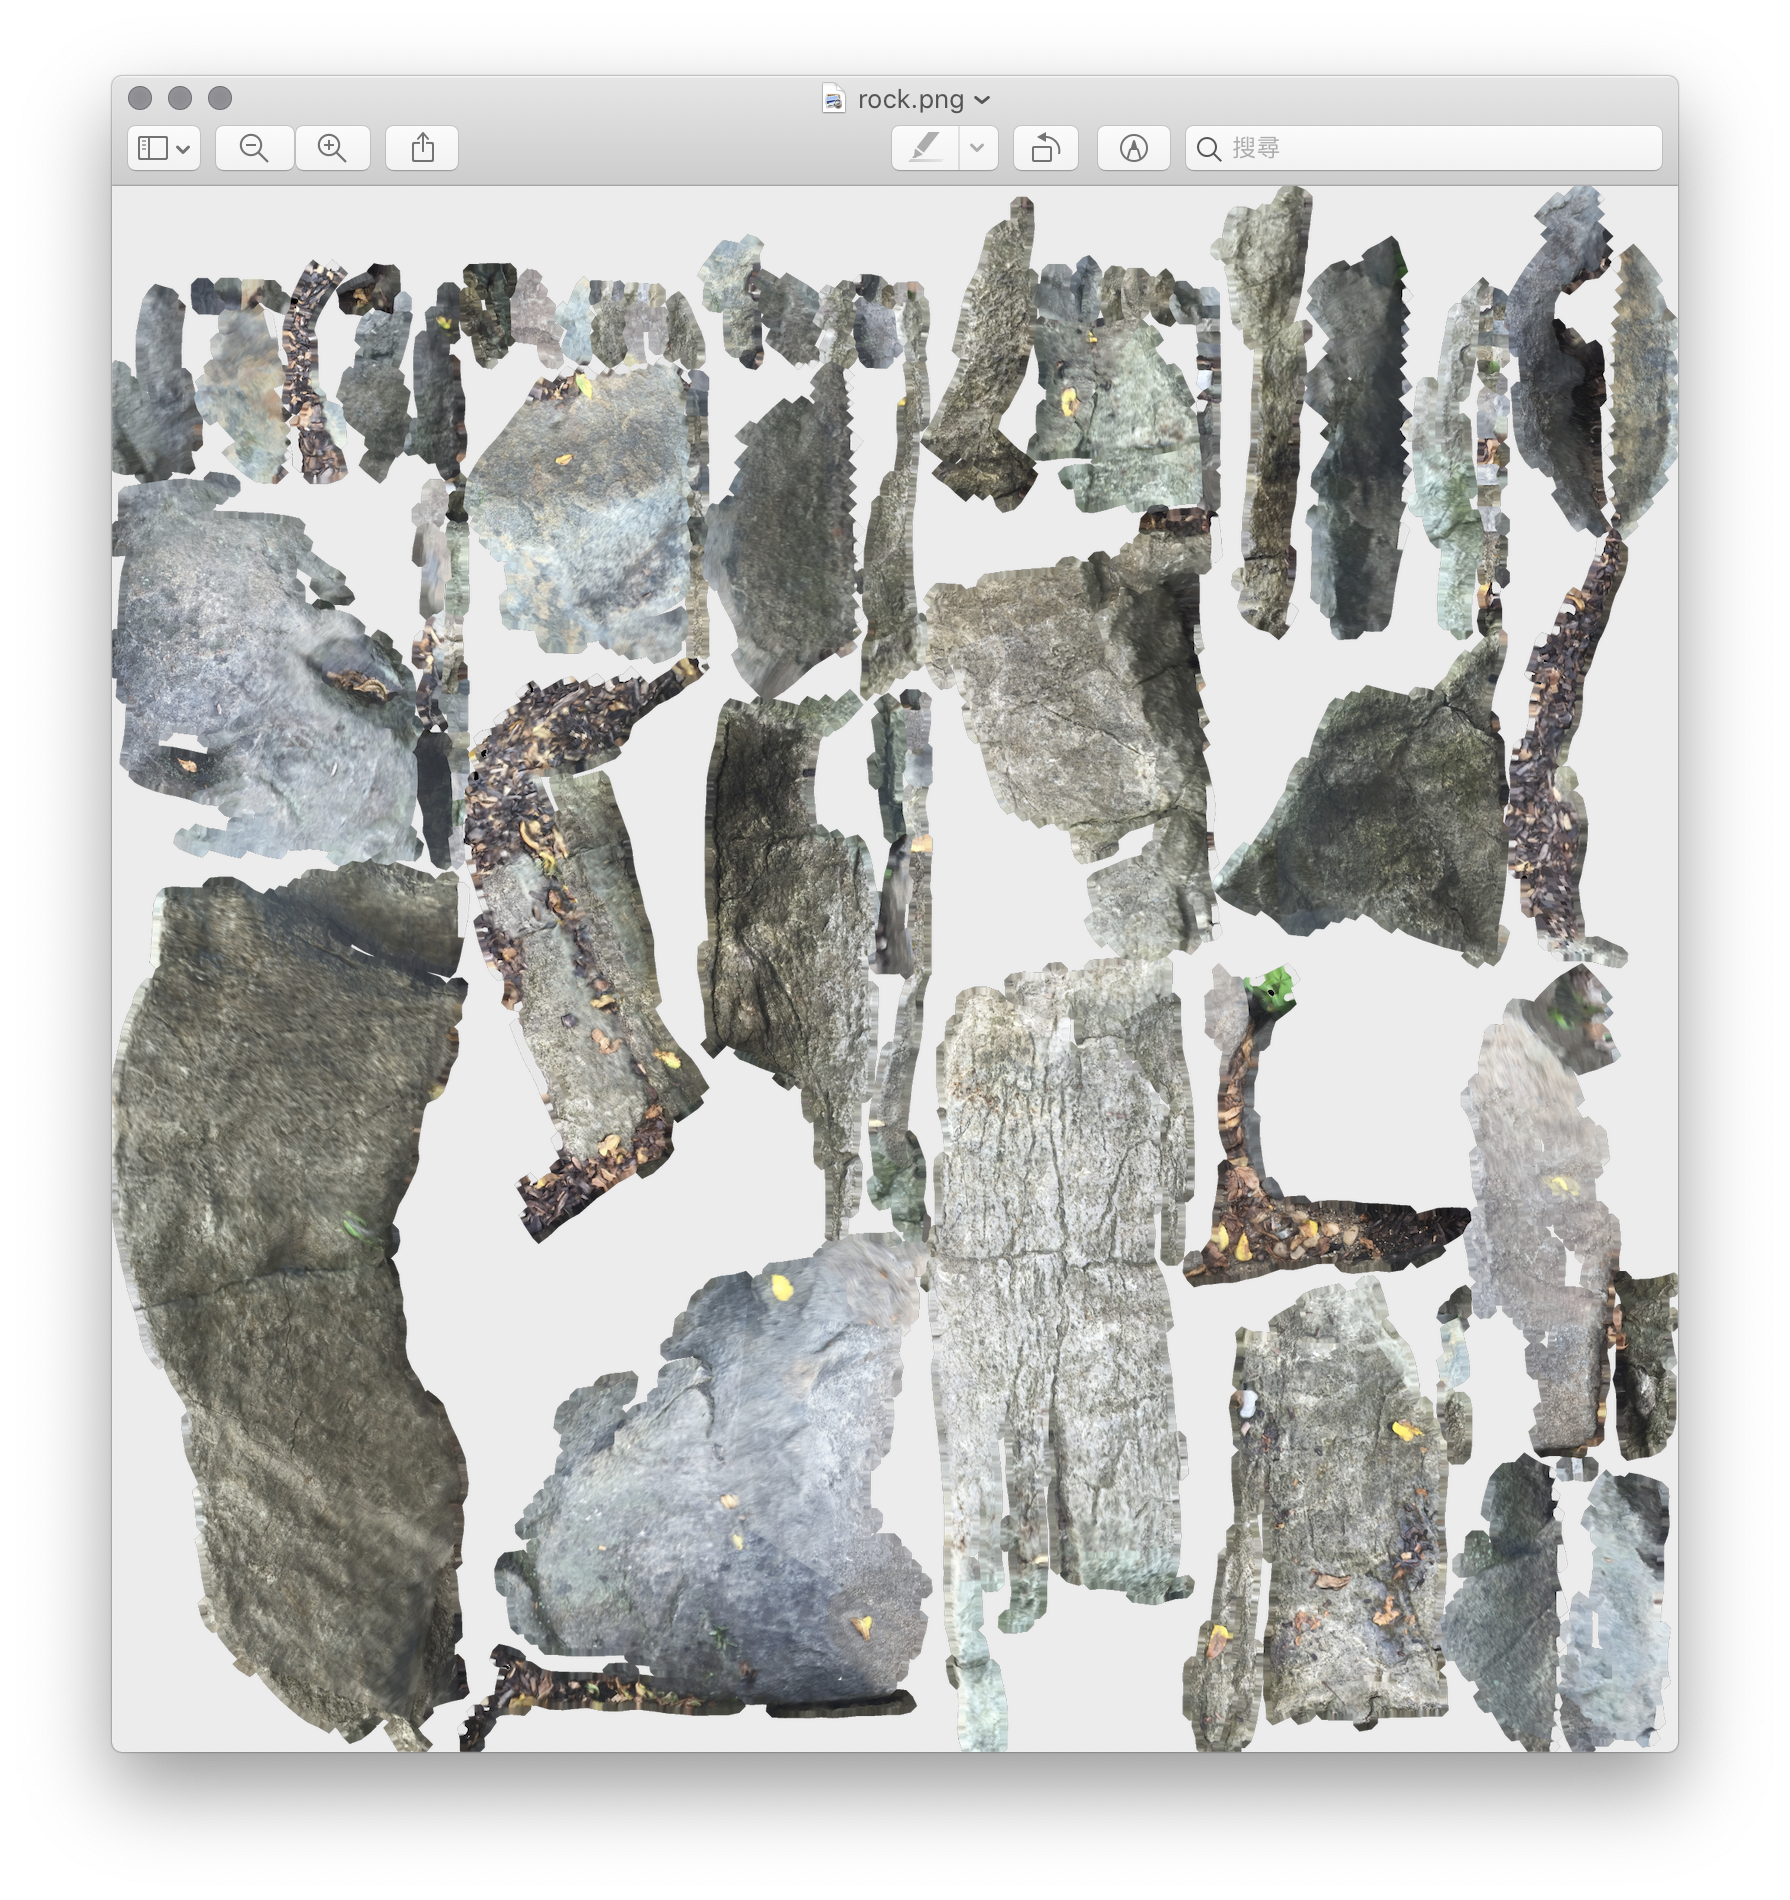
\includegraphics{/Volumes/Macintosh HD (Sierra)/Users/yue/Documents/GitHub/2019-2020-autumn-semester/SE-344/submissions/ass4-ng-x/report/report.assets/rock_mapping.png}
\caption{}
\end{figure}

这里,采用了一些拼贴的办法来减小贴图文件的大小。

\hypertarget{header-n215}{%
\subparagraph{模型读取}\label{header-n215}}

WaveFront 格式的读取方式比照 Assignment \#3 实现。

Ply 格式的读取基于 tinyply 的包装函数实现。

\begin{quote}
\texttt{.obj} 格式的读取器参见
\texttt{./3-bomb/ObjLoader/ObjLoaderWrapped.hpp}。

\texttt{.ply} 格式的读取器参见
\texttt{./3-bomb/PlyLoader/PlyReaderWrapped.hpp}。
\end{quote}

留意到因为要实现贴图,\texttt{.ply}
格式的读取器需要同时读取定点位置、法向量方向、贴图 UV 坐标。

\hypertarget{header-n234}{%
\subparagraph{坐标转换}\label{header-n234}}

经过文本编辑器打开分析我下载的 \texttt{.ply}
文件,发现它并没有提供贴图所用的 UV 坐标,而是提供了 ST 坐标。

ST 坐标系和 UV
坐标系是对同一数据的不同表示。幸好他们可以通过这一公式简单的转化:

\(s = u\)、\(t = 1 - v\)。

所以做一次变换即可。

\hypertarget{header-n246}{%
\subparagraph{贴图读取}\label{header-n246}}

参见第一部分中的「材质加载」部分。

\hypertarget{header-n254}{%
\subparagraph{模型绘制}\label{header-n254}}

要在绘制三角形的时候,同时将物体表面的贴图和法向量(用于光照计算)绘制出来,只需要在调用
\texttt{glVertex} 之前调用 \texttt{glNormal} 指定法向量方向,并调用
\texttt{glTexCoords} 指定贴图坐标即可。

另外,别忘了用 \texttt{glBindTexture} 和
\texttt{glEnable(GL\_TEXTURE\_2D)} 来启用材质哦。

\hypertarget{header-n263}{%
\subparagraph{光照绘制}\label{header-n263}}

参见 Assignment \#3 中的光照绘制。

特别地,为了模拟手电筒的效果,我们会在一定范围内随机地扰动光照位置,模拟手持手电筒的颤抖效果,增强真实感。

特别要注意,假如我们不提供法线方向,则光线效果十分微弱,完全没有立体感;但我们提供了这一信息之後,光线模拟的结果就相对比较真实了。

\begin{figure}
\centering
\includegraphics{/Users/yue/Documents/GitHub/2019-2020-autumn-semester/SE-344/submissions/ass4-ng-x/report/report.assets/normal_and_no_normal.png}
\caption{}
\end{figure}

\hypertarget{header-n276}{%
\subparagraph{背景贴图}\label{header-n276}}

为了实现暗室之中反射的效果,我们在这个房间周围放置四个平面,在未贴图的情况下如下图所示:

\begin{figure}
\centering
\includegraphics{/Users/yue/Documents/GitHub/2019-2020-autumn-semester/SE-344/submissions/ass4-ng-x/report/report.assets/wall_no_mapping.png}
\caption{}
\end{figure}

然後,我们只需要在四面上贴上提供的暗室图片材质就行了。

比照第二部分「雾气弥漫」中的背景绘制实现即可。

\hypertarget{header-n284}{%
\paragraph{第四部分:佛祖保佑}\label{header-n284}}

\hypertarget{header-n286}{%
\subparagraph{环境搭建}\label{header-n286}}

由于此部分和上一节的环境一致(还是在那个房间里),因此将其直接拷贝过来,并且稍微把摄影机视角抬高一点,以体现佛祖的神圣性。

另外,为了使得各个方向来的光线可以分辨,这里我们在三个等距方向上放置了三盏
RGB 灯光。这样方向就能直观地通过颜色的不同来区分了。

\hypertarget{header-n293}{%
\subparagraph{模型加载}\label{header-n293}}

事实上,这里最难办的部分就是模型加载了。鉴于分辨率最高的模型文件大小达到了数十
MiB,在测试机器上需要耗费数十秒钟加载,因此同步的读取显然不现实。

因此我们采取一个折衷的办法:在开始绘制之前,仅仅加载最低分辨率的模型,并开启一个子线程加载中等分辨率的模型;在中等分辨率模型加载线程完成加载後,会开启一个新线程来加载高分辨率的模型\ldots\ldots 以此类推,程序能够在後台按照顺序加载由低到高分辨率的模型。

由于程序在 Windows 环境下编译,因此使用 Windows 风格的多线程 API。

在此之前需要先引入 \texttt{Windows.h}。

\begin{Shaded}
\begin{Highlighting}[]
\NormalTok{DWORD WINAPI fun( LPVOID lpParameter );}
\end{Highlighting}
\end{Shaded}

以这种形式定义的函数即可被作为一个子线程执行。

\begin{Shaded}
\begin{Highlighting}[]
\NormalTok{CreateThread( }\KeywordTok{nullptr}\NormalTok{, }\DecValTok{0}\NormalTok{, foo, }\KeywordTok{nullptr}\NormalTok{, }\DecValTok{0}\NormalTok{, }\KeywordTok{nullptr}\NormalTok{ );}
\end{Highlighting}
\end{Shaded}

调用 \texttt{CreateThread} 函数即可启动子线程啦。

\hypertarget{header-n313}{%
\subparagraph{模型绘制}\label{header-n313}}

跟第三部分基本类似,只是这里不需要贴图,只需要调整模型材质和色泽即可。

\hypertarget{header-n316}{%
\paragraph{第五部分:超监督}\label{header-n316}}

所谓的「超监督」就是依次调度上面四个子程序的外壳程序。同时她还负责背景音乐的播放。

\hypertarget{header-n320}{%
\subparagraph{音频读取}\label{header-n320}}

每个叙事阶段都有特定的背景音乐,有一些场景还有多种音效的混合。

因此为了实现混合音频的播放,这里使用了 \texttt{System.Windows.Media}
中提供的 \texttt{MediaPlayer} 对象来承担音频播放的任务。

使用前请务必 \texttt{using\ System.Windows.Media}。

在产生场景切换时,音乐调度器会收到通知,并调整启用的音轨。

\hypertarget{header-n330}{%
\subparagraph{程序执行}\label{header-n330}}

超监督本身没有场景绘制的功能,因此其中出现的资源都是 Photoshop
画出来的。

她通过调用 \texttt{System.Diagnostics.Process.Start}
函数来实现唤起子程序的功能,并在程序结束时回调主线程进入下一阶段。

使用前请务必 \texttt{using\ System.Diagnostics}。

\hypertarget{header-n724}{%
\subparagraph{依赖}\label{header-n724}}

主程序使用 C\# 书写,依赖于 Microsoft .NET Framework 4.7.2。

此外,需要 \texttt{wmp.dll} 以实现音频播放功能。

\hypertarget{header-n342}{%
\subsubsection{问题和解决}\label{header-n342}}

\hypertarget{header-n346}{%
\paragraph{ST 坐标系和 UV 坐标系}\label{header-n346}}

ply 格式中可能使用 ST 坐标系来描述贴图,也可能使用 UV 坐标系。

这两种描述方法只是坐标轴的原点和方向不同,本质上并无区别。

在读取时一定要细心留意这两种不同的情况并分别处理,否则就会产生贴图错误。

\hypertarget{header-n351}{%
\paragraph{Blend Mode 和 Depth Test}\label{header-n351}}

深度测试在大部分时候都应当开启,除非希望手动渲染半透明的物体或使用非默认的混合模式,不希望
OpenGL 自动将被遮挡物体从渲染管线中移除。这种时候还是应当禁用它。

\hypertarget{header-n357}{%
\paragraph{MediaPlayer 和 SoundPlayer}\label{header-n357}}

MediaPlayer 由 \texttt{System.Windows.Media} 提供,而 SoundPlayer 则是由
\texttt{System.Media} 提供。

它们之间的差别(之一)是 SoundPlayer
不支持多个实例同时活跃,较早的播放实例会被自动停止。

由于在本例中需要用到音轨的混合,因此使用 MediaPlayer 而不用
SoundPlayer。

\begin{quote}
另外的解决方案是直接 \texttt{@DllImport("winmm.dll")} 并直接调用
DirectSound 的 C/C++ 风格的接口。

具体的实现参见 \texttt{./hypervisor/SimultaneousMediaPlayer.cs} 文件。

实际测试发现在部分虚拟机环境下并不能正常工作,因此不推荐使用。
\end{quote}

\hypertarget{header-n370}{%
\paragraph{SOIL 里的坑}\label{header-n370}}

在 Debug 的过程中,留意到 SOIL
在读取部分类型的贴图文件时,会出现图片倒置的错误,即旋转了 180
度的问题。

为了尽量减少程序的负担,采取直接将原始图片旋转 180 度的策略来修正问题。

STBI 库未发现此类问题。

\hypertarget{header-n740}{%
\paragraph{机能限制}\label{header-n740}}

鉴于测试机器并没有独立显卡,且 OpenGL 实现是 VMWare
虚拟机提供的,性能堪忧。因此程序在绘制最高分辨率佛像模型的时候会出现严重的掉帧,绘制速率甚至不到
10 帧每秒。

因此佛像的旋转速度相应地调快了些,以适应显示效果。

另外,程序中大部分用于流程控制的代码都并非基于经过的帧数而是执行程序以来的真实时间。因此掉帧不会对程序流程产生影响。

\hypertarget{header-n735}{%
\subsubsection{笔记}\label{header-n735}}

自第九周(2019 年 11 月 7 日)以来的笔记参见 \texttt{./notes} 目录下的
Markdown 和 TeX 文件。

\hypertarget{header-n755}{%
\subsubsection{致谢}\label{header-n755}}

\hypertarget{header-n756}{%
\paragraph{Documentations}\label{header-n756}}

\begin{itemize}
\item
  \href{https://learnopengl.com}{learnopengl.com}
\item
  \href{http://www.opengl-tutorial.org}{opengl-tutorial.org}
\end{itemize}

\hypertarget{header-n775}{%
\paragraph{Third-Party Libraries}\label{header-n775}}

\begin{itemize}
\item
  \href{http://glew.sourceforge.net}{\textbf{glew}}, the OpenGL
  extension wrangler library
\item
  \href{https://www.glfw.org}{\textbf{glfw}}, multi-platform library for
  OpenGL
\item
  \href{http://freeglut.sourceforge.net}{\textbf{freeGLUT}}, open-source
  alternative to GLUT
\item
  \href{https://github.com/syoyo/tinyobjloader/}{\textbf{tinyobj}}, tiny
  but powerful wavefront obj loader
\item
  \href{https://github.com/ddiakopoulos/tinyply}{\textbf{tinyply}},
  c++11 ply 3d mesh format importer \& exporter
\item
  \href{https://github.com/paralin/soil}{\textbf{SOIL}}, simple OpenGL
  image library
\item
  \href{https://glm.g-truc.net}{\textbf{glm}}, OpenGL mathematics
  library 
\end{itemize}

\hypertarget{header-n816}{%
\paragraph{SE-344 staff}\label{header-n816}}

\end{document}
